\subsection{Lian's summary}

\subsubsection{Random parameters and random labels}
\paragraph{Summary}
\begin{enumerate}
\item On Cifar100, the training accuracy is bigger than $99.9\%$ if we randomly generate the parameters in the input layer (8 channels)
\item On Cifar100, the training accuracy (on training+validation datasets) is $94\%$ if we randomly generate the labels and train the input layers (8 channels)
\item Deep neural networks easily fit random data. More experiments are shown in a paper. It means that the effective capacity of neural networks is sufficient for memorizing the data.
%\item Layers consisting of convolution following by pooling naturally
%become frequency selective and translation invariant when assigned random weights.
%\item The networks with random Gaussian weights perform a distance-preserving embedding of
%the data, with a special treatment for in-class and out-of-class data.
\end{enumerate}

\paragraph{Numerical results: random parameters}
Denote $f$ be the input image (size of $32*32$ in Cifar datasets), $\hat{\xi}$ is the convolutional layer with random parameters and $\hat{A}$ is the linear layer with random parameters, which are both not trained, and $\hat{\sigma}$ is the activation function.
We have two models:
\begin{itemize}
\item Model I
\begin{align}
	\hat{g}^1 & = \hat{\sigma}(\hat{A} (f))  \label{random conv eq} \\
	P & = LR(\hat{g}^1)
\end{align}
\item Model II 
\begin{align}
\hat{g}^1 & = \hat{\sigma}(\hat{\xi} (f))  \label{random conv eq} \\
P & = LR(\hat{g}^1)
\end{align}
\item Model III
\begin{align}
\hat{g}^1 & = \hat{\sigma}(BN(\hat{\xi} (Aug(f))))  \label{random conv eq} \\
P & = LR(\hat{g}^1)
\end{align}
\end{itemize}

We consider Kaiming He's initialization\cite{he2015delving} strategy to sample the random parameters of the convolutional layer $\hat{\xi}$ from uniform distribution $\mathcal{U}(-b,b)$, where $b$ is given by
\begin{equation}
	b = gain * \sqrt{\frac{3}{c_{in}*n_{in}*n_{in}}}
\end{equation}
where $c_{in}$ is the number of input channels, $n_{in}*n_{in}$ is size of each input channel and $gain$ depends on the the activation function, which is recommended in Pytorch as follows:
\begin{table}[H]
	\caption{gain values of different activation functions}
	\label{gain}
	\begin{center}
			\begin{tabular}{|c|c|}
				\hline
				Activation funtions & gain
				\tabularnewline \hline
				Linear/Identity & $1$
				\tabularnewline \hline
				Sigmoid   & $1$				 
				\tabularnewline \hline
				ReLu   & $\sqrt{2}	$	
				\tabularnewline \hline
				PReLu   & $\sqrt{\frac{2}{1+slope^2}}	$
				\tabularnewline \hline			 
			\end{tabular} 
	\end{center}
\end{table}

\begin{table}[H]
	\caption{Parametric ReLU (PReLU) performance on MNIST}
	\begin{center}
		\begin{tabular}{|c|c|c|}
			\hline
			$\alpha$ in PReLU & Training accuracy & Test accuracy
			\tabularnewline \hline
			1     & 93.4433  & 92.5000
			\tabularnewline \hline
			0.9   & 93.8050  & 92.7000				 
			\tabularnewline \hline
			0.8   & 96.0900	 & 95.3600
			\tabularnewline \hline
			0.7   & 97.2250  & 96.6900
			\tabularnewline \hline	
			0.6   & 99.2817  & 97.3400
			\tabularnewline \hline	
			0.5   & 100.0000 & 98.0500
			\tabularnewline \hline
			0.4   & 100.0000 & 98.1500
			\tabularnewline \hline	
			0.3   & 100.0000 & 98.2400
			\tabularnewline \hline	
			0.2   & 100.0000 & 98.2400
			\tabularnewline \hline	
			0.1   & 100.0000 & 98.4300
			\tabularnewline \hline	
			0.0   & 100.0000 & 98.3800
			\tabularnewline \hline		 
		\end{tabular} 
	\end{center}
\end{table}

MNIST, CIFAR
Input image: 3 * 32 *32 

Size of A: (3 * 32 * 32) * (N * 32 * 32 )

Size of LR: (N * 32 * 32 ) * 10 or 100 


INAGENET
Input image: 3 * 256 *256 

Size of A: (3 * 256 * 256) * (N *  256 * 256)

Size of LR: (N *  256 * 256 ) * 1000
 
 \paragraph{Model I: random fully connected layer}
\begin{table}[H]
	\caption{Training accuracy on Cifar100: Model I with $\hat{\sigma}=ReLU$}
	\begin{center}
		\resizebox{\textwidth}{!}{
			\begin{tabular}{|c|c|c|c|c|c|c|}
				\hline
				Input size for LR&  Test 1 & Test 2 &  Test 3 & Test 4 & Test 5 & Average
				\tabularnewline \hline
					3072 = 3 *32*32&99.9533&99.9550&99.9433&99.9550&99.9583&99.9530
					
					\tabularnewline \hline 
					
					4096 = 4 *32*32&99.9650&99.9700&99.9700&99.9650&99.9650&99.9670
					
					\tabularnewline \hline 
					
					5120 = 5 *32*32&99.9700&99.9717&99.9700&99.9700&99.9700&99.9703
					
					\tabularnewline \hline 
					
					6144 = 6 *32*32&99.9700&99.9700&99.9717&99.9717&99.9700&99.9707
					
					\tabularnewline \hline 
					
					7168 = 7 *32*32&99.9717&99.9717&99.9700&99.9717&99.9700&99.9710
					
					\tabularnewline \hline 
					
					8192 = 8 *32*32&99.9717&99.9717&99.9717&99.9700&99.9717&99.9714
					
					\tabularnewline \hline 
					
					9216 = 9 *32*32&99.9700&99.9717&99.9717&99.9700&99.9717&99.9710
					
					\tabularnewline \hline 
					
					10240 = 10 *32*32&99.9717&99.9717&99.9717&99.9717&99.9717&99.9717
					
					\tabularnewline \hline 

			\end{tabular} 
		}
	\end{center}
\end{table}

\begin{table}[H]
	\caption{Training accuracy on Cifar10: Model I with $\hat{\sigma}=ReLU$}
	\begin{center}
		\resizebox{\textwidth}{!}{
			\begin{tabular}{|c|c|c|c|c|c|c|c|}
				\hline
				Input size for LR&  Test 1 & Test 2 &  Test 3 & Test 4 & Test 5 & Average 
				\tabularnewline \hline
				3072 = 3 *32*32&60.8650&60.7700&61.1150&61.0933&61.1317&60.9950
				
				\tabularnewline \hline 
				
				5120 = 5 *32*32&74.5350&74.7100&74.7517&74.3033&74.4400&74.5480
				
				\tabularnewline \hline 
				
				10240 = 10 *32*32&99.7117&99.7033&99.7017&99.6800&99.7267&99.7047
				
				\tabularnewline \hline 
				
				15360 = 15 *32*32&99.9983&99.9967&99.9983&99.9950&100.0000&99.9977
				
				\tabularnewline \hline 
				
				20480 = 20 *32*32&100.0000&100.0000&100.0000&99.9983&99.9983&99.9993
				
				\tabularnewline \hline 
				
				25600 = 25 *32*32&100.0000&100.0000&100.0000&100.0000&100.0000&100.0000
				
				\tabularnewline \hline 
				
				30720 = 30 *32*32&100.0000&100.0000&100.0000&100.0000&100.0000&100.0000
				
				\tabularnewline \hline 
				
				35840 = 35 *32*32&100.0000&100.0000&100.0000&100.0000&100.0000&100.0000
				
				\tabularnewline \hline 
				
				40960 = 40 *32*32&100.0000&100.0000&100.0000&100.0000&100.0000&100.0000
				
				\tabularnewline \hline 
				
			\end{tabular} 
		}
	\end{center}
\end{table} 

 \paragraph{Model II: random convolutional layer}
\begin{table}[H]
	\caption{Training accuracy on ImageNet: Model II with $\hat{\sigma}=ReLU$}
	\begin{center}
		\resizebox{\textwidth}{!}{
			\begin{tabular}{|c|c|c|c|c|c|c|}
				\hline
				Input size for LR&  Test 1 & Test 2 &  Test 3 & Test 4 & Test 5 & Average
				\tabularnewline \hline
				196,608 = 3 *256*256& 95.2571  & 94.9728 &  95.3812&&&
				\tabularnewline \hline 
				262,144 = 4 *256*256& 98.6554  &&&&&
				\tabularnewline \hline 
				327,680 = 5 *256*256& 98.7532 &&&&&
				\tabularnewline \hline 
			\end{tabular} 
		}
	\end{center}
\end{table} 
 
\begin{table}[H]
	\caption{Training accuracy on Cifar100: Model II with $\hat{\sigma}=ReLU$}
	\begin{center}
		\resizebox{\textwidth}{!}{
			\begin{tabular}{|c|c|c|c|c|c|c|}
				\hline
				Input size for LR&  Test 1 & Test 2 &  Test 3 & Test 4 & Test 5 & Average
				\tabularnewline \hline
					3072 = 3 *32*32&79.4500&81.1517&97.1383&96.3117&89.5233&88.7150
					
					\tabularnewline \hline 
					
					4096 = 4 *32*32&98.9717&96.8517&95.1217&98.3650&97.6633&97.3947
					
					\tabularnewline \hline 
					
					5120 = 5 *32*32&99.7450&96.0617&98.1983&99.2117&99.2817&98.4997
					
					\tabularnewline \hline 
					
					6144 = 6 *32*32&99.9033&97.5550&99.0233&98.6183&99.9117&99.0023
					
					\tabularnewline \hline 
					
					7168 = 7 *32*32&99.7550&99.8650&99.9533&99.5967&99.5583&99.7457
					
					\tabularnewline \hline 
					
					8192 = 8 *32*32&99.7817&99.9683&99.9150&99.9550&99.8167&99.8873
					
					\tabularnewline \hline 
					
					9216 = 9 *32*32&99.8733&99.8533&99.9333&99.9483&99.9500&99.9116
					
					\tabularnewline \hline 
					
					10240 = 10 *32*32&99.9600&99.9483&99.9567&99.9583&99.9250&99.9497
					
					\tabularnewline \hline  
			\end{tabular} 
		}
	\end{center}
\end{table}
 
\begin{table}[H]
	\caption{Training accuracy on Cifar10: Model II with $\hat{\sigma}=ReLU$}
	\begin{center}
		\resizebox{\textwidth}{!}{
			\begin{tabular}{|c|c|c|c|c|c|c|c|}
				\hline
				Input size for LR&  Test 1 & Test 2 &  Test 3 & Test 4 & Test 5 & Average 
				\tabularnewline \hline
				3072 = 3 *32*32&48.0300&47.3517&49.8233&46.8650&47.1383&47.8417
				
				\tabularnewline \hline 	
				
				5120 = 5 *32*32&64.4733&60.7550&63.1050&60.3600&58.8317&61.5050
				
				
				\tabularnewline \hline 
				
				10240 = 10 *32*32&87.8200&83.2317&88.6333&83.6383&89.6933&86.6033
				
				
				\tabularnewline \hline 
				
				15360 = 15 *32*32&94.7167&95.2767&92.1033&95.7183&90.4150&93.6460
				
				\tabularnewline \hline 
				
				20480 = 20 *32*32&99.5717&96.2867&97.3233&98.0367&98.9650&98.0367
				
				
				\tabularnewline \hline 
				
				25600 = 25 *32*32&98.8783&97.3650&99.7300&97.2917&98.8050&98.4140
				
				\tabularnewline \hline 
				
				30720 = 30 *32*32&99.6717&99.8433&99.1417&99.5367&99.1783&99.4743
				
				\tabularnewline \hline 
				
				35840 = 35 *32*32&99.8967&99.9733&99.2300&98.6667&99.7283&99.4990
				
				\tabularnewline \hline 
				
				40960 = 40 *32*32&99.9300&99.9000&99.9750&99.7100&99.9683&99.8967
				
				\tabularnewline \hline 
			\end{tabular} 
		}
	\end{center}
\end{table} 
 
\begin{table}[H]
	\caption{Training accuracy on Cifar10: Model II with $\hat{\sigma}=ReLU$ (more detail)}
	\begin{center}
		\resizebox{\textwidth}{!}{
			\begin{tabular}{|c|c|c|c|c|c|c|c|}
				\hline
				Input size for LR&  Test 1 & Test 2 &  Test 3 & Test 4 & Test 5 & Average 
				\tabularnewline \hline
				3072 = 3 *32*32&48.0300&47.3517&49.8233&46.8650&47.1383&47.8417
				
				\tabularnewline \hline 
				
				4096 = 4 *32*32&56.7550&53.5600&60.7483&54.7633&54.2767&56.0207
				
				\tabularnewline \hline 
				
				5120 = 5 *32*32&64.4733&60.7550&63.1050&60.3600&58.8317&61.5050
				
				\tabularnewline \hline 
				
				6144 = 6 *32*32&66.8350&69.2233&69.7617&65.7967&70.7800&68.4793
				
				\tabularnewline \hline 
				
				7168 = 7 *32*32&75.4983&79.7833&73.3950&75.5067&74.3300&75.7027
				
				\tabularnewline \hline 
				
				8192 = 8 *32*32&78.2000&76.1533&76.5517&76.6567&75.5650&76.6253
				
				\tabularnewline \hline 
				
				9216 = 9 *32*32&85.6283&76.7517&74.6183&79.4350&87.4650&80.7797
				
				\tabularnewline \hline 
				
				10240 = 10 *32*32&87.8200&83.2317&88.6333&83.6383&89.6933&86.6033
				
				\tabularnewline \hline 
				
				11264 = 11 *32*32&92.6867&94.9533&86.8783&91.2450&83.5900&89.8707
				
				\tabularnewline \hline 
				
				12288 = 12 *32*32&87.9033&89.6683&90.3950&89.5400&86.0467&88.7107
				
				\tabularnewline \hline 
				
				13312 = 13 *32*32&96.3633&91.2550&95.8867&97.3350&93.6983&94.9077
				
				\tabularnewline \hline 
				
				14336 = 14 *32*32&98.6633&91.3750&94.7250&93.3917&90.1400&93.6590
				
				\tabularnewline \hline 
				
				15360 = 15 *32*32&94.7167&95.2767&92.1033&95.7183&90.4150&93.6460
				
				\tabularnewline \hline 
				
				16384 = 16 *32*32&97.1200&91.4600&95.1833&90.7650&96.4800&94.2017
				
				\tabularnewline \hline 
				
				17408 = 17 *32*32&98.0433&97.7500&97.0467&98.5350&97.5683&97.7887
				
				\tabularnewline \hline 
				
				18432 = 18 *32*32&97.9717&95.7883&97.0800&98.0850&98.0600&97.3970
				
				\tabularnewline \hline 
				
				19456 = 19 *32*32&99.9300&99.4317&97.4833&97.0167&98.5050&98.4733
				
				\tabularnewline \hline 
				
				20480 = 20 *32*32&99.5717&96.2867&97.3233&98.0367&98.9650&98.0367
				
				\tabularnewline \hline 
				
				21504 = 21 *32*32&95.5067&98.2767&99.1200&98.2317&95.2467&97.2764
				
				\tabularnewline \hline 
				
				22528 = 22 *32*32&97.3883&99.2517&99.8583&99.8933&99.1117&99.1007
				
				\tabularnewline \hline 
				
				23552 = 23 *32*32&97.3233&99.5717&99.1533&97.8083&98.9017&98.5517
				
				\tabularnewline \hline 
				
				24576 = 24 *32*32&99.5417&99.9333&98.4350&99.3700&97.6367&98.9833
				
				\tabularnewline \hline 
				
				25600 = 25 *32*32&98.8783&97.3650&99.7300&97.2917&98.8050&98.4140
				
				\tabularnewline \hline 
				
				26624 = 26 *32*32&98.8983&99.7517&98.9750&99.3433&98.2667&99.0470
				
				\tabularnewline \hline 
				
				27648 = 27 *32*32&99.8000&99.4550&99.4817&99.9433&99.6550&99.6670
				
				\tabularnewline \hline 
				
				28672 = 28 *32*32&98.0667&99.5717&99.5683&99.5383&98.6117&99.0713
				
				\tabularnewline \hline 
				
				29696 = 29 *32*32&99.9200&98.8050&98.0717&99.5967&99.5567&99.1900
				
				\tabularnewline \hline 
				
				30720 = 30 *32*32&99.6717&99.8433&99.1417&99.5367&99.1783&99.4743
				
				\tabularnewline \hline 
				
				31744 = 31 *32*32&99.9750&98.9017&99.7033&99.8417&99.2267&99.5297
				
				\tabularnewline \hline 
				
				32768 = 32 *32*32&98.2067&99.7150&99.4900&99.8617&98.6700&99.1887
				
				\tabularnewline \hline 
				
				33792 = 33 *32*32&99.7983&99.7733&99.0950&98.8767&98.7833&99.2653
				
				\tabularnewline \hline 
				
				34816 = 34 *32*32&95.9617&99.6050&99.9633&99.5900&99.1200&98.8480
				
				\tabularnewline \hline 
			\end{tabular} 
		}
	\end{center}
\end{table}
 
 
\begin{table}[H]
	\caption{Training accuracy on Cifar100: Model III with different $\hat{\sigma}$}
	\label{case1: random conv}
	\begin{center}
		\resizebox{\textwidth}{!}{
			\begin{tabular}{|c|c|c|c|c|c|c|}
				\hline
				input size for LR&  $\sigma=I$ & $\sigma=Sigmoid$ &  $\sigma=ReLU$ & $\sigma=PReLU(a=0.01)$ & $\sigma=PReLU(a=0.1)$ & $\sigma=PReLU(a=-1)$
				\tabularnewline \hline
				%$(Huang)\hat{g}^1$  &  95.2 & 8192\tabularnewline \hline
				$3072=3*32*32$  &  49.8233  & 34.1300 & 69.8917 & 80.825   & 66.6333 & 65.1267
				\tabularnewline \hline
				$4096=4*32*32$  &  44.7550  & 31.4300 & 84.7917 & 76.0700  &94.4833&  67.5783
				\tabularnewline \hline
				$5120=5*32*32$  &  55.6200  & 35.1467 & 92.2917 & 91.8433  &99.7317 &   99.6733
				\tabularnewline \hline
				$6144=6*32*32$  &  50.3050  & 35.7700 & 99.7450 & 99.8717  &97.2783&  97.8767
				\tabularnewline \hline
				$7168=7*32*32$  &  62.5033  & 46.0883 & 99.0450 & 99.7733  &99.9500&  99.9733
				\tabularnewline \hline
				$8192=8*32*32$  &  60.5050  & 37.5767 & 99.9600 & 99.9933  &99.9167&  99.8917
				\tabularnewline \hline
				$9216=9*32*32$  &  65.7700  & 35.5250 & 99.9617 & 99.9933  &99.9617&   99.9917
				\tabularnewline \hline
				$10240=10*32*32$&  55.4367  & 40.6433 & 99.9950 & 99.9933  &99.9717&  99.995
				\tabularnewline \hline
				$>10240$        & around 65 & around 40 & $>99.99$& $>99.99$&$>99.99$& $>99.99$
				\tabularnewline \hline
			\end{tabular} 
		}
	\end{center}
\end{table}

\begin{table}[H]
	\caption{Training accuracy on Cifar10: Model III with different $\hat{\sigma}$}
	\begin{center}
		\resizebox{\textwidth}{!}{
			\begin{tabular}{|c|c|c|c|c|c|c|c|}
				\hline
				input size for LR&  $\sigma=I$ & $\sigma=Sigmoid$ &  $\sigma=ReLU$ & $\sigma=PReLU(a=0.01)$ & $\sigma=PReLU(a=0.1)$ & $\sigma=PReLU(a=-1)$
				\tabularnewline \hline
				%$(Huang)\hat{g}^1$  &  95.2 & 8192\tabularnewline \hline
				$3072=3*32*32$  &  37.0300  & 35.6933 & 39.325    & 39.7700 &  &
				\tabularnewline \hline
				$4096=4*32*32$  &  37.3867  & 36.4867  & 39.9183   & 44.4617 & &
				\tabularnewline \hline
				$5120=5*32*32$  &  39.5583  & 37.4867  & 54.0567   & 49.6150 & &
				\tabularnewline \hline
				$6144=6*32*32$  &  38.3083  & 38.4683  & 57.0517   & 58.0633 & &
				\tabularnewline \hline
				$7168=7*32*32$  &  39.2117  & 39.8050  & 57.8367   & 65.4500 & &
				\tabularnewline \hline
				$8192=8*32*32$  &  39.5567  & 41.3833  & 64.5850    & 62.7417 & &
				\tabularnewline \hline
				$9216=9*32*32$  &  39.1150  & 40.9500  & 67.9933   & 70.9617 & &
				\tabularnewline \hline
				$10240=10*32*32$&  39.6850  & 38.3017  & 69.4217   & 73.5983 & &
				\tabularnewline \hline
				$11264=11*32*32$  & 41.0633   & 41.6183  & 71.2050 & 71.6667& &
				\tabularnewline \hline
				$12288=12*32*32$  & 39.7650   & 39.8017  & 85.0500 & 81.3350  & &
				\tabularnewline \hline
				$13312=13*32*32$  & 39.9983   &  43.4217 & 79.0333 & 84.9600 & &
				\tabularnewline \hline
				$14336=14*32*32$  & 39.6800   & 41.8933  & 77.0650  & 75.4400 & &
				\tabularnewline \hline
				$15360=15*32*32$& 39.4400   &   41.8483 & 85.9883   & 86.7567& &
				\tabularnewline \hline
				$16384=16*32*32$  & 40.2400   & 41.8300  & 94.8733 & 94.9183  & &
				\tabularnewline \hline
				$17408=17*32*32$  &    &   & 85.6983   &  & &
				\tabularnewline \hline
				$18432=18*32*32$  &    &   & 91.2150  &  & &
				\tabularnewline \hline
				$19456=19*32*32$  &    &   & 92.6283   &  & &
				\tabularnewline \hline
				$20480=20*32*32$&    &   & 95.5317  &  & &
				\tabularnewline \hline
				$21504=21*32*32$  &    &   & 95.5033   &  & &
				\tabularnewline \hline
				$22528=22*32*32$  &    &   & 97.9950   &  & &
				\tabularnewline \hline
				$23552=23*32*32$  &    &   & 96.1267  &  & &
				\tabularnewline \hline
				$24576=24*32*32$  &    &   & 96.6367   &  & &
				\tabularnewline \hline
				$25600=25*32*32$&    &   & 95.5133  &  & &
				\tabularnewline \hline
				$26624=26*32*32$  &    &   & 95.9267   &  & &
				\tabularnewline \hline
				$27648=27*32*32$  &    &   & 94.8983  &  & &
				\tabularnewline \hline
				$28672=28*32*32$  &    &   & 98.7300  &  & &
				\tabularnewline \hline
				$29696=29*32*32$  &    &   & 98.8367   &  & &
				\tabularnewline \hline
				$30720=30*32*32$&    &   &  99.3833  &  & &
				\tabularnewline \hline
				$31744=31*32*32$  &    &  & 99.3650  &  & &
				\tabularnewline \hline
				$32768=32*32*32$  &    &  & 99.7283  &  & &
				\tabularnewline \hline
				$33792=33*32*32$  &    &   & 99.8317  &  & &
				\tabularnewline \hline
				$34816=34*32*32$  &    &   & 99.8461  &  & &
				\tabularnewline \hline
			\end{tabular} 
		}
	\end{center}
\end{table}
\begin{figure}[!htpt]
	\centering
	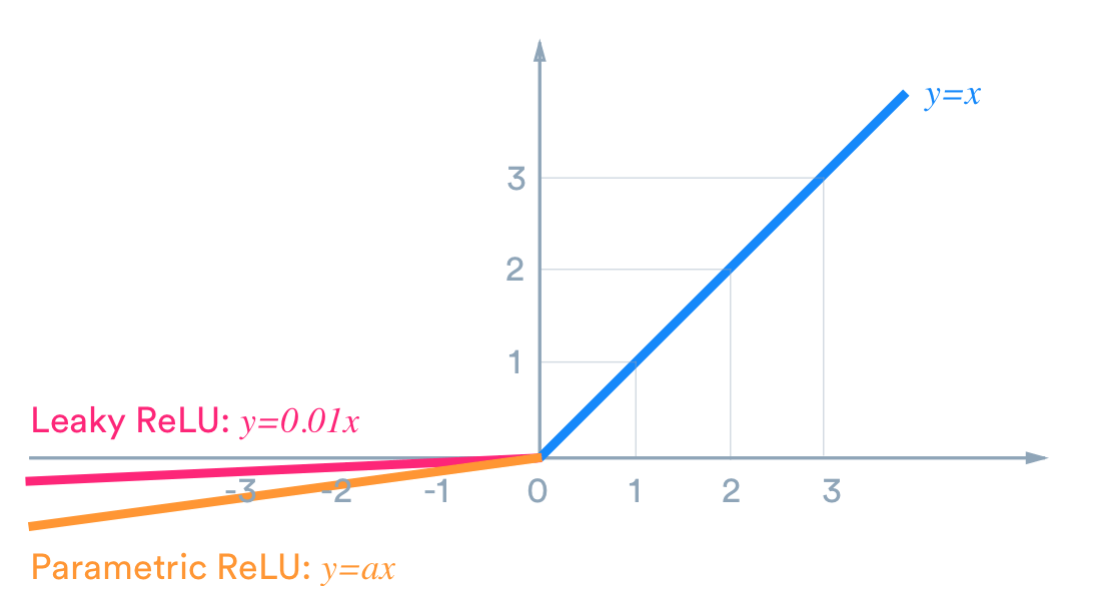
\includegraphics[width=0.8\textwidth]{LeakyReLU.png}
	\caption{LeakyReLU}.
	\label{LeakyReLU}
\end{figure}
Further, if we also randomize the labels, the training accuracy on Cifar100 (training+validation datasets) is $92\%$, which is shown in Table \ref{case1: random labels}
\begin{table}[H]
	\caption{On Cifar100: Random labels and input layer}
	\label{case1: random labels}
	\begin{center}
		\resizebox{\textwidth}{!}{
			\begin{tabular}{|c|c|c|c|c|}
				\hline
				$\Phi(\cdot)$&  training accuracy
				& input size for LR\tabularnewline
				\hline
				$\hat{g}^1$  &  92.9126 & 
				8192\tabularnewline
				\hline																
			\end{tabular} 
		}
	\end{center}
\end{table}
A paper did more experiments on random data, the main results are shown in Fig. \ref{randomdata}
\begin{figure}[!htpt]
	\centering
	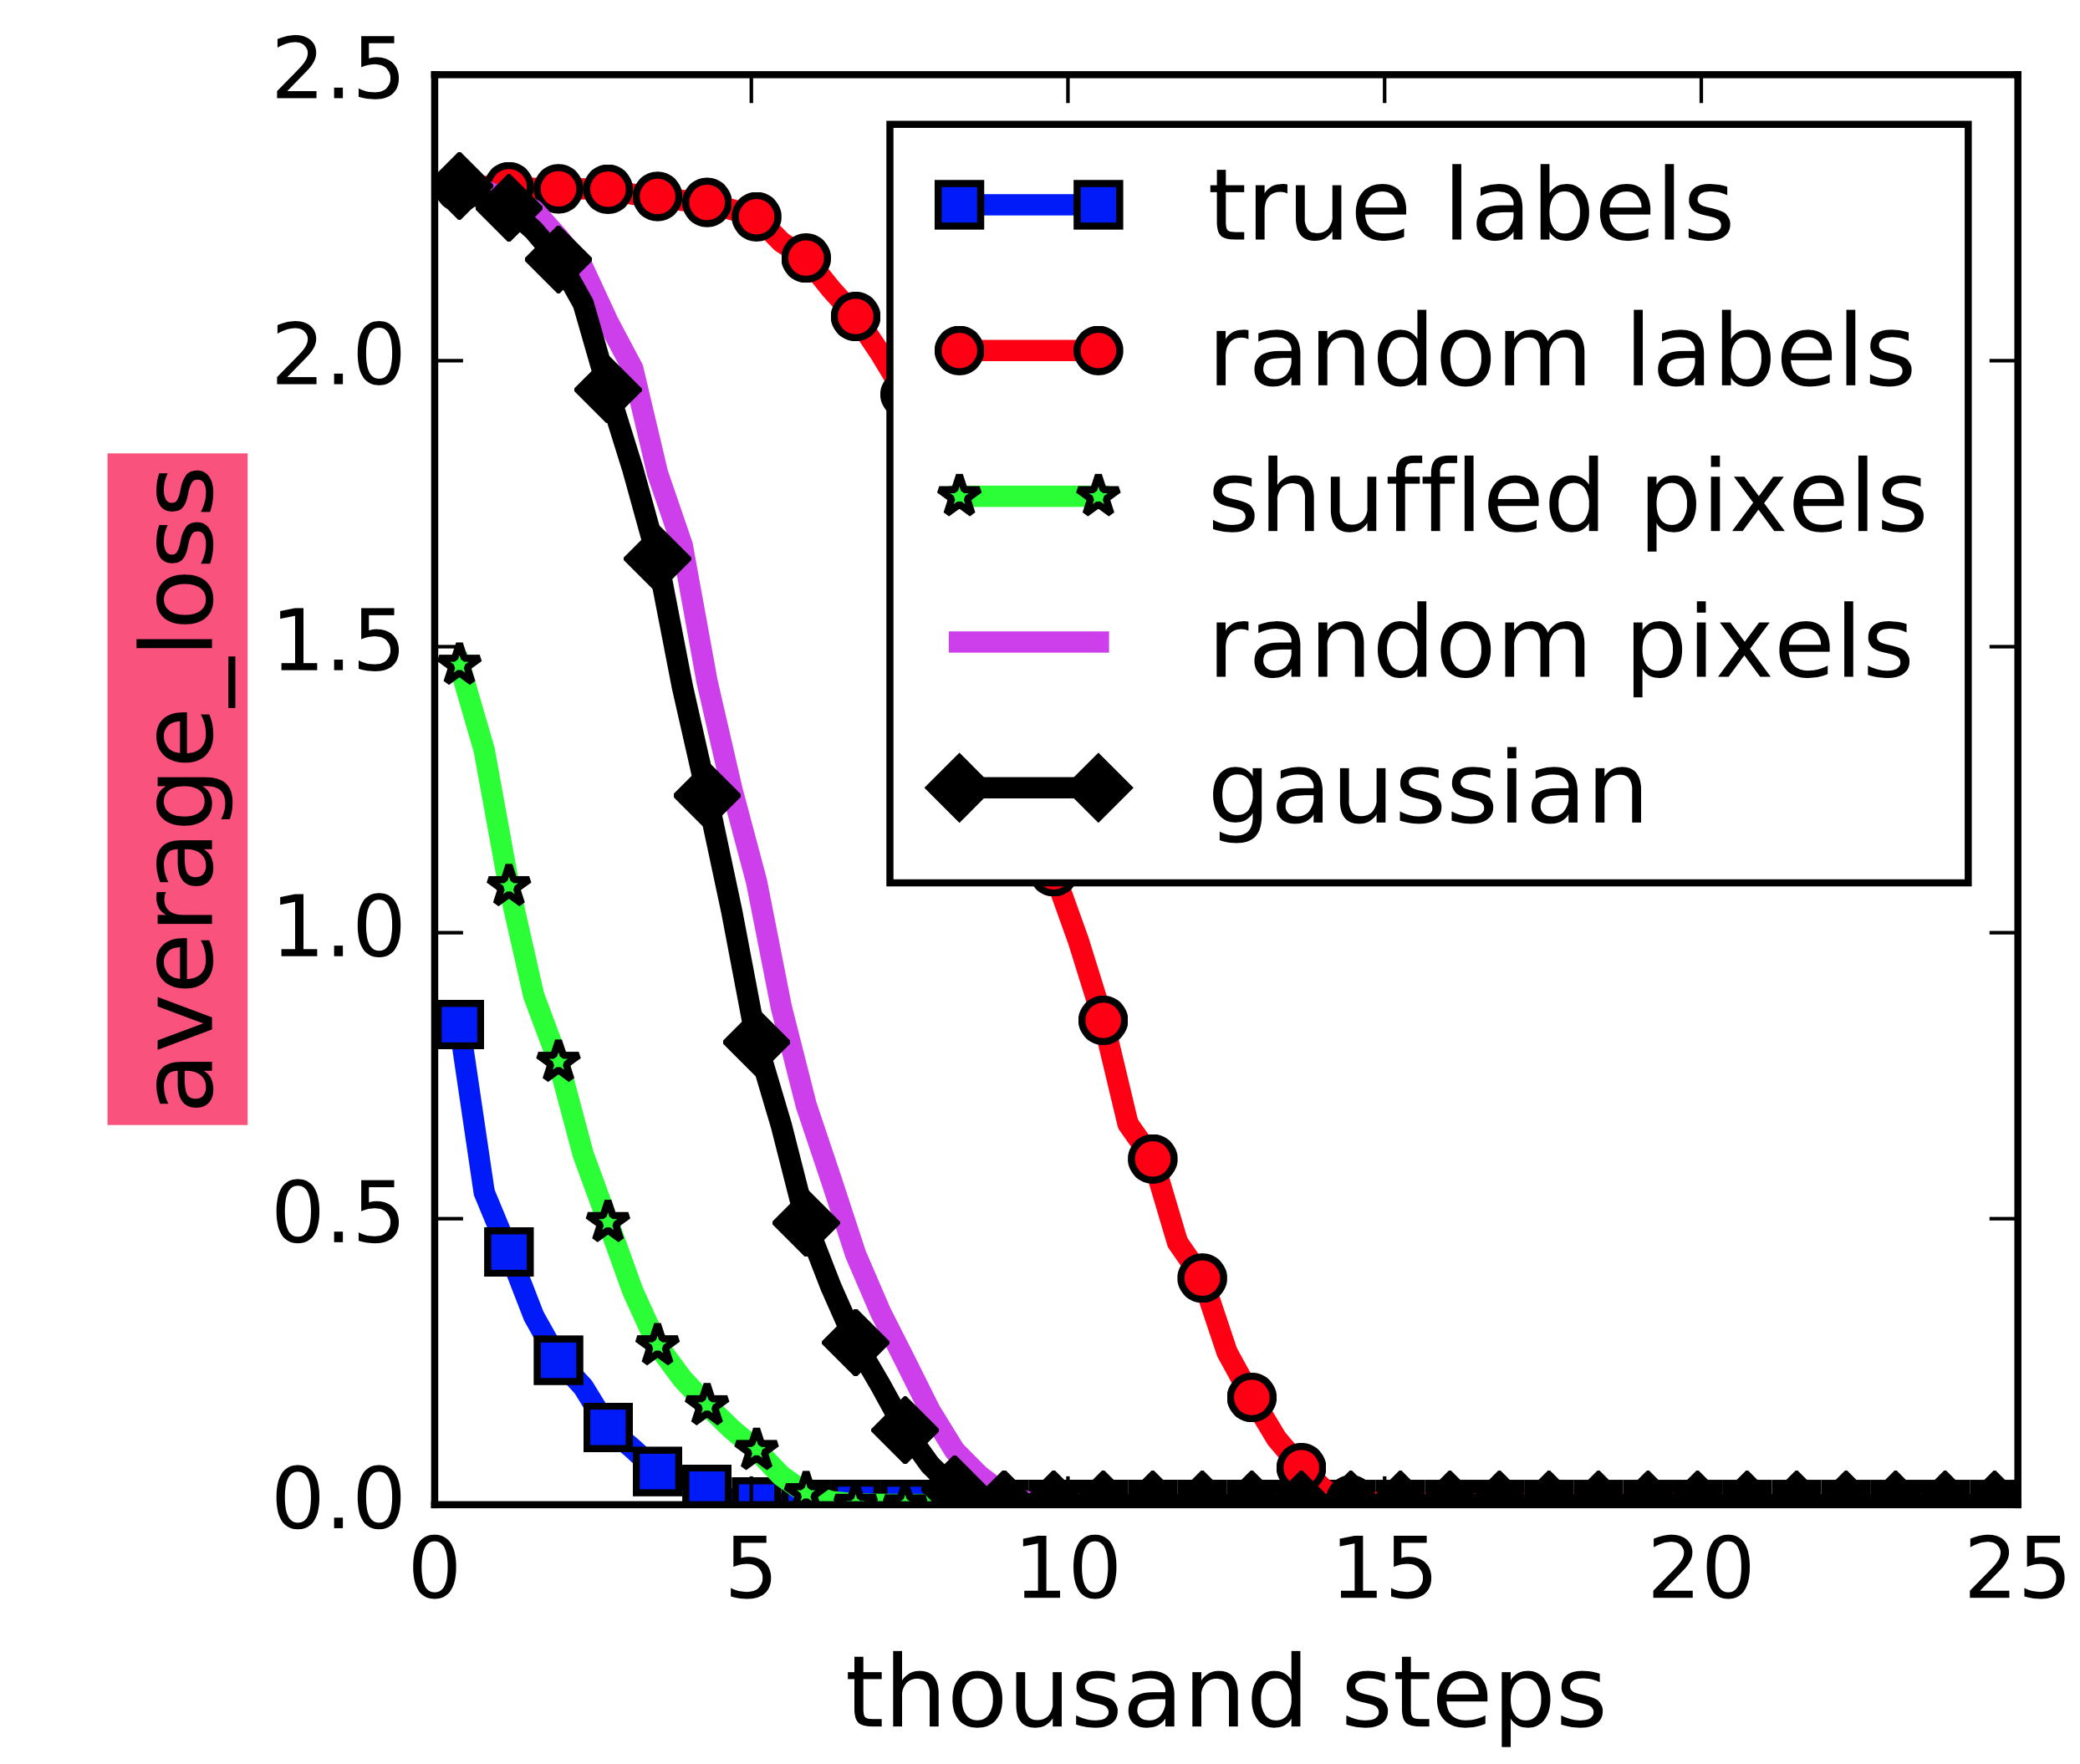
\includegraphics[width=0.8\textwidth]{randomdata.png}
	\caption{Fitting random labels and random pixels on CIFAR10 with AlexNet.
		(1) True labels: the original dataset without modification.
		(2) Random labels: all the labels are replaced with random ones.
		(3) Shuffled pixels: a random permutation of the pixels is chosen and then the same permutation is applied to all the images in both training and test set.
		(4) Random pixels: a different random permutation is applied to each image independently.
		(5) Gaussian:A Gaussian distribution(with matching mean and variance to the original image
		dataset) is used to generate random pixels for each image.}
	\label{randomdata}
\end{figure}
\subsubsection{Linearly separable on Cifar10}
\paragraph{Summary}
\begin{enumerate}
\item The smallest dimension of linearly separable new data, which is generated from Cifar10 raw data by nonliner transformations(convolution+BN+ReLU), is 8192.
\item Discussion: Linear separation is related to number of data, number of features, number of classes, number of data in each class.
\end{enumerate}

\paragraph{Numerical results}

\begin{itemize}
	\item Case 1: size 8192
\end{itemize}



\begin{align}
u^1 & MgNet(f; J=1, \nu_1=2)  \\
u^{6} & = \tilde{\Pi}_1^6(u^1) \\
p & = LR(u^6)
\end{align}
\begin{table}[H]
	\caption{ResNet18 on CIFAR-10: $J=1,\nu_1=2,c_f^1=c_u^1=8$, with the last average pooling}
	\label{case1 with 1 grids_cifar10}
	\begin{threeparttable}
		
		\begin{center}
			\resizebox{\textwidth}{!}{
				\begin{tabular}{|c|c|c|c|}
					\hline
					$\Phi(\cdot)$ & ResNet training accuracy & linear model training  accuracy
					& input size for LR\tabularnewline
					\hline
					$u^1$  &  25.7291  &  99.9933  &
					8192\tabularnewline
					\hline											
				\end{tabular} 
				
			}
		\end{center}
		
	\end{threeparttable}
\end{table}

\begin{align}
u^1 & = MgNet(f; J=1, \nu_1=2)  \\
p & = LR(u^1)
\end{align}


\begin{table}[H]
	\caption{ResNet18 on CIFAR-10: $J=1,\nu_1=2,c_f^1=c_u^1=8$, without the last average pooling}
	\label{case1: mgnet without last pooling}
	\begin{center}
		\resizebox{\textwidth}{!}{
			\begin{tabular}{|c|c|c|c|c|}
				\hline
				$\Phi(\cdot)$      & mgnet training accuracy & linear model training accuracy
				&  input size for LR
				\tabularnewline
				\hline
				$u^1$             &  68.808                                   & 99.997 
					          & 8192\tabularnewline
				\hline												
			\end{tabular} 
		}
		
	\end{center}
\end{table}



\begin{itemize}
\item Case 2: size 4096
\end{itemize}
\begin{align}
u^1 & = MgNet(f; J=1, \nu_1=2)  \\
u^{2} & = {\Pi}_1^2(u^1) \\
p & = LR(u^2)
\end{align}
\begin{table}[!htbp]
	\caption{ResNet18 on CIFAR-10: $J=1,\nu_1=2,c_f^1=c_u^1=8$, with stride 2 pooling (16 channels)}
	\begin{center}
		\resizebox{\textwidth}{!}{
			\begin{tabular}{|c|c|c|c|c|}
				\hline
				$\Phi(\cdot)$      & ResNet training accuracy & linear model training accuracy
				& input size for LR
				\tabularnewline
				\hline
				$u^2$             & 67.856                            & 82.345
				 		          & 4096\tabularnewline
				\hline												
			\end{tabular} 
		}
	\end{center}
\end{table}



\begin{itemize}
	\item Case 3: size 2048
\end{itemize}
\begin{table}[H]
	\caption{ResNet18 on CIFAR-10: $J=1,\nu_1=2,c_f^1=c_u^1=8$, with stride 2 pooling (8 channels)}
	\begin{center}
		\resizebox{\textwidth}{!}{
			\begin{tabular}{|c|c|c|c|c|}
				\hline
				$\Phi(\cdot)$      & ResNet training accuracy & linear model training accuracy
				& input size for LR
				\tabularnewline
				\hline
				$u^2$             &  67.54                                   & 73.455
				 		          & 2048\tabularnewline
				\hline												
			\end{tabular} 
		}
		
	\end{center}
\end{table}

\subsubsection{On Cifar100: linear transformations}
Given the linearly separable data $(x_i,y_i), i=1,2,...,6000$ generated from the Cifar100 raw data, we test various linear transformations followed by a logistic regression on the input data. As an example, we take the data with input size 2048 ($x_i\in \mathcal{R^2048}$).
\begin{itemize}
\item Case 1: $P_1(x_i;w_1)$ = $A_{100\times 2048}x_i$; $y_i$=Maxout($P_1$)\\
\item Case 2: $P_2(x_i;w_2)$ = $A_{100\times 256}A_{256\times 512}A_{512\times 1024}A_{1024\times 2048}x_i$; $y_i$=Maxout($P_2$)\\
\end{itemize}


\begin{table}[H]
	\caption{On Cifar100: linear transformations + logistic regression on linearly separable data (dimension 2048).}
	\begin{center}
		\resizebox{\textwidth}{!}{
			\begin{tabular}{|c|c|c|}
				\hline
				Case      &  training accuracy & validation accuracy
				\tabularnewline
				\hline
				1               & 99.998           & 16.17
				\tabularnewline				\hline
				2               & 99.96           & 15.26
				\tabularnewline
				\hline											
			\end{tabular} 
		}
	\end{center}
\end{table}


\subsubsection{A modified ResNet: activation function only imposed on the first grid}
In this subsection, we only impose activation functions (RuLU) on the first grid.
\begin{table}[H]
	\caption{ResNet18 on CIFAR-100: $J=4,\nu_1=\nu_2=\nu_3=\nu_4=2,c_f^1=c_u^1=64 (nonlinear),~ c_u^2=128,~c_u^3=256,~c_u^4=512$}
	\begin{center}
		\resizebox{\textwidth}{!}{
			\begin{tabular}{|c|c|c|}
				\hline
				Model      &  training accuracy & validation accuracy
				\tabularnewline
				\hline
				Best validation model           & 73.308           & 61.13
				\tabularnewline				\hline
				Last epoch model                & 93.286           & 54.12
				\tabularnewline
				\hline												
			\end{tabular} 
		}
	\end{center}
\end{table}
\begin{table}[H]
	\caption{ResNet18 on CIFAR-100: $J=4,\nu_1=\nu_2=\nu_3=\nu_4=2,c_f^1=c_u^1=64 (nonlinear),~ c_u^2=c_u^3=c_u^4=512$}
	\begin{center}
		\resizebox{\textwidth}{!}{
			\begin{tabular}{|c|c|c|}
				\hline
				Model      &  training accuracy & validation accuracy
				\tabularnewline
				\hline
				Best validation model           & 73.048           & 61.58
				\tabularnewline				\hline
				Last epoch model                & 92.75            & 56.45
				\tabularnewline
				\hline												
			\end{tabular} 
		}
	\end{center}
\end{table}

%\subsubsection{A modified ResNet: color independent kernels}
\subsubsection{Best model on ImageNet}
\paragraph{Summary}
We test Efficientnet-B7 on ImageNet. The training accuracy is $95.87\%$ and the validation accuracy is $84.31\%$.	

\subsubsection{Linear Model}

\begin{table}[!h]
	\begin{center}
		\begin{tabular}{|l|cc|c|}
			\hline
			Model   					& Accuracy  & \# Parameters & Reproduce Accuracy \\	
			\hline\hline
			ResNet18       				& 74.45		& 11M  	&   77.43\\ \hline
			ResNet18-$A^l$ 				& 74.46 	& 8.1M 	&   77.46\\ \hline
			ResNet18-$B^l$ 				& 72.78  	& 9.8M 	&\\ \hline
			ResNet18-$A^l$-$B^l$ 		& 72.56  	& 6.7M 	&\\ \hline
			iResNet18       			& 74.33 	& 11M  	&\\ \hline
			iResNet18-$A^l$ 			& 74.51 	& 8.1M  &\\ \hline
			iResNet18-$B^l$ 			& 72.67 	& 9.8M  &\\ \hline
			iResNet18-$A^l$-$B^l$ 		& 72.81  	& 6.6M 	&\\ \hline
			ResNet34       				& 77.20 	& 21M &\\ \hline
			ResNet34-$A^l$ 				& 77.24 	& 13M &\\ \hline
			ResNet34-$B^l$ 				& 75.31		& 15M &\\ \hline
			ResNet34-$A^l$-$B^l$ 		& 74.79   	& 6.7M &\\ \hline
			iResNet34       			& 77.25 	& 21M &\\ \hline
			iResNet34-$A^l$ 			& 77.40 	& 13M   &\\ \hline
			iResNet34-$B^l$ 			& 75.36 	& 15M  &\\ \hline
			iResNet34-$A^l$-$B^l$ 		& 75.82 	& 6.7M  & \\ \hline
		\end{tabular}
	\end{center}
	\caption{The accuracy and number of parameters for ResNet on Cifar100.}
\end{table}

\begin{table}[!h]
	\begin{center}
		\begin{tabular}{|l|c|c|c|}
			\hline
			Model   					& Accuracy	& Accuracy(TenCrop) & \# Parameters \\	
			\hline\hline
			ResNet18       				&  70.23  	& 72.75	  &  11.7M  		\\ 
			\hline
			ResNet18-$A^l$ 				&  69.45	& 71.86  &  8.6M   		\\ 
			\hline
			iResNet18       			&  70.46	& 72.88	  &  11.7M			\\ 
			\hline
			iResNet18-$A^l$ 			&  69.78	& 71.82  &  8.6M			\\ 
			\hline
			ResNet34       				&  74.61  & 76.33  &  21.8M	\\ 
			\hline
			ResNet34-$A^l$ 				&  72.13	& 74.40   &  13.6M    \\ 
			\hline
			iResNet34       			&  74.38	& 76.17  &  21.8M \\ 
			\hline
			iResNet34-$A^l$ 			&  72.20	& 74.61   &  13.6M \\ 
			\hline
		\end{tabular}
	\end{center}
	\caption{The accuracy and number of parameters for ResNet on ImageNet without/with TenCrop.}
\end{table}

TenCrop: Crop the given Image into four corners and the central crop plus the flipped version of these (horizontal flipping is used by default)






\begin{figure}[!htpt]
	\centering
	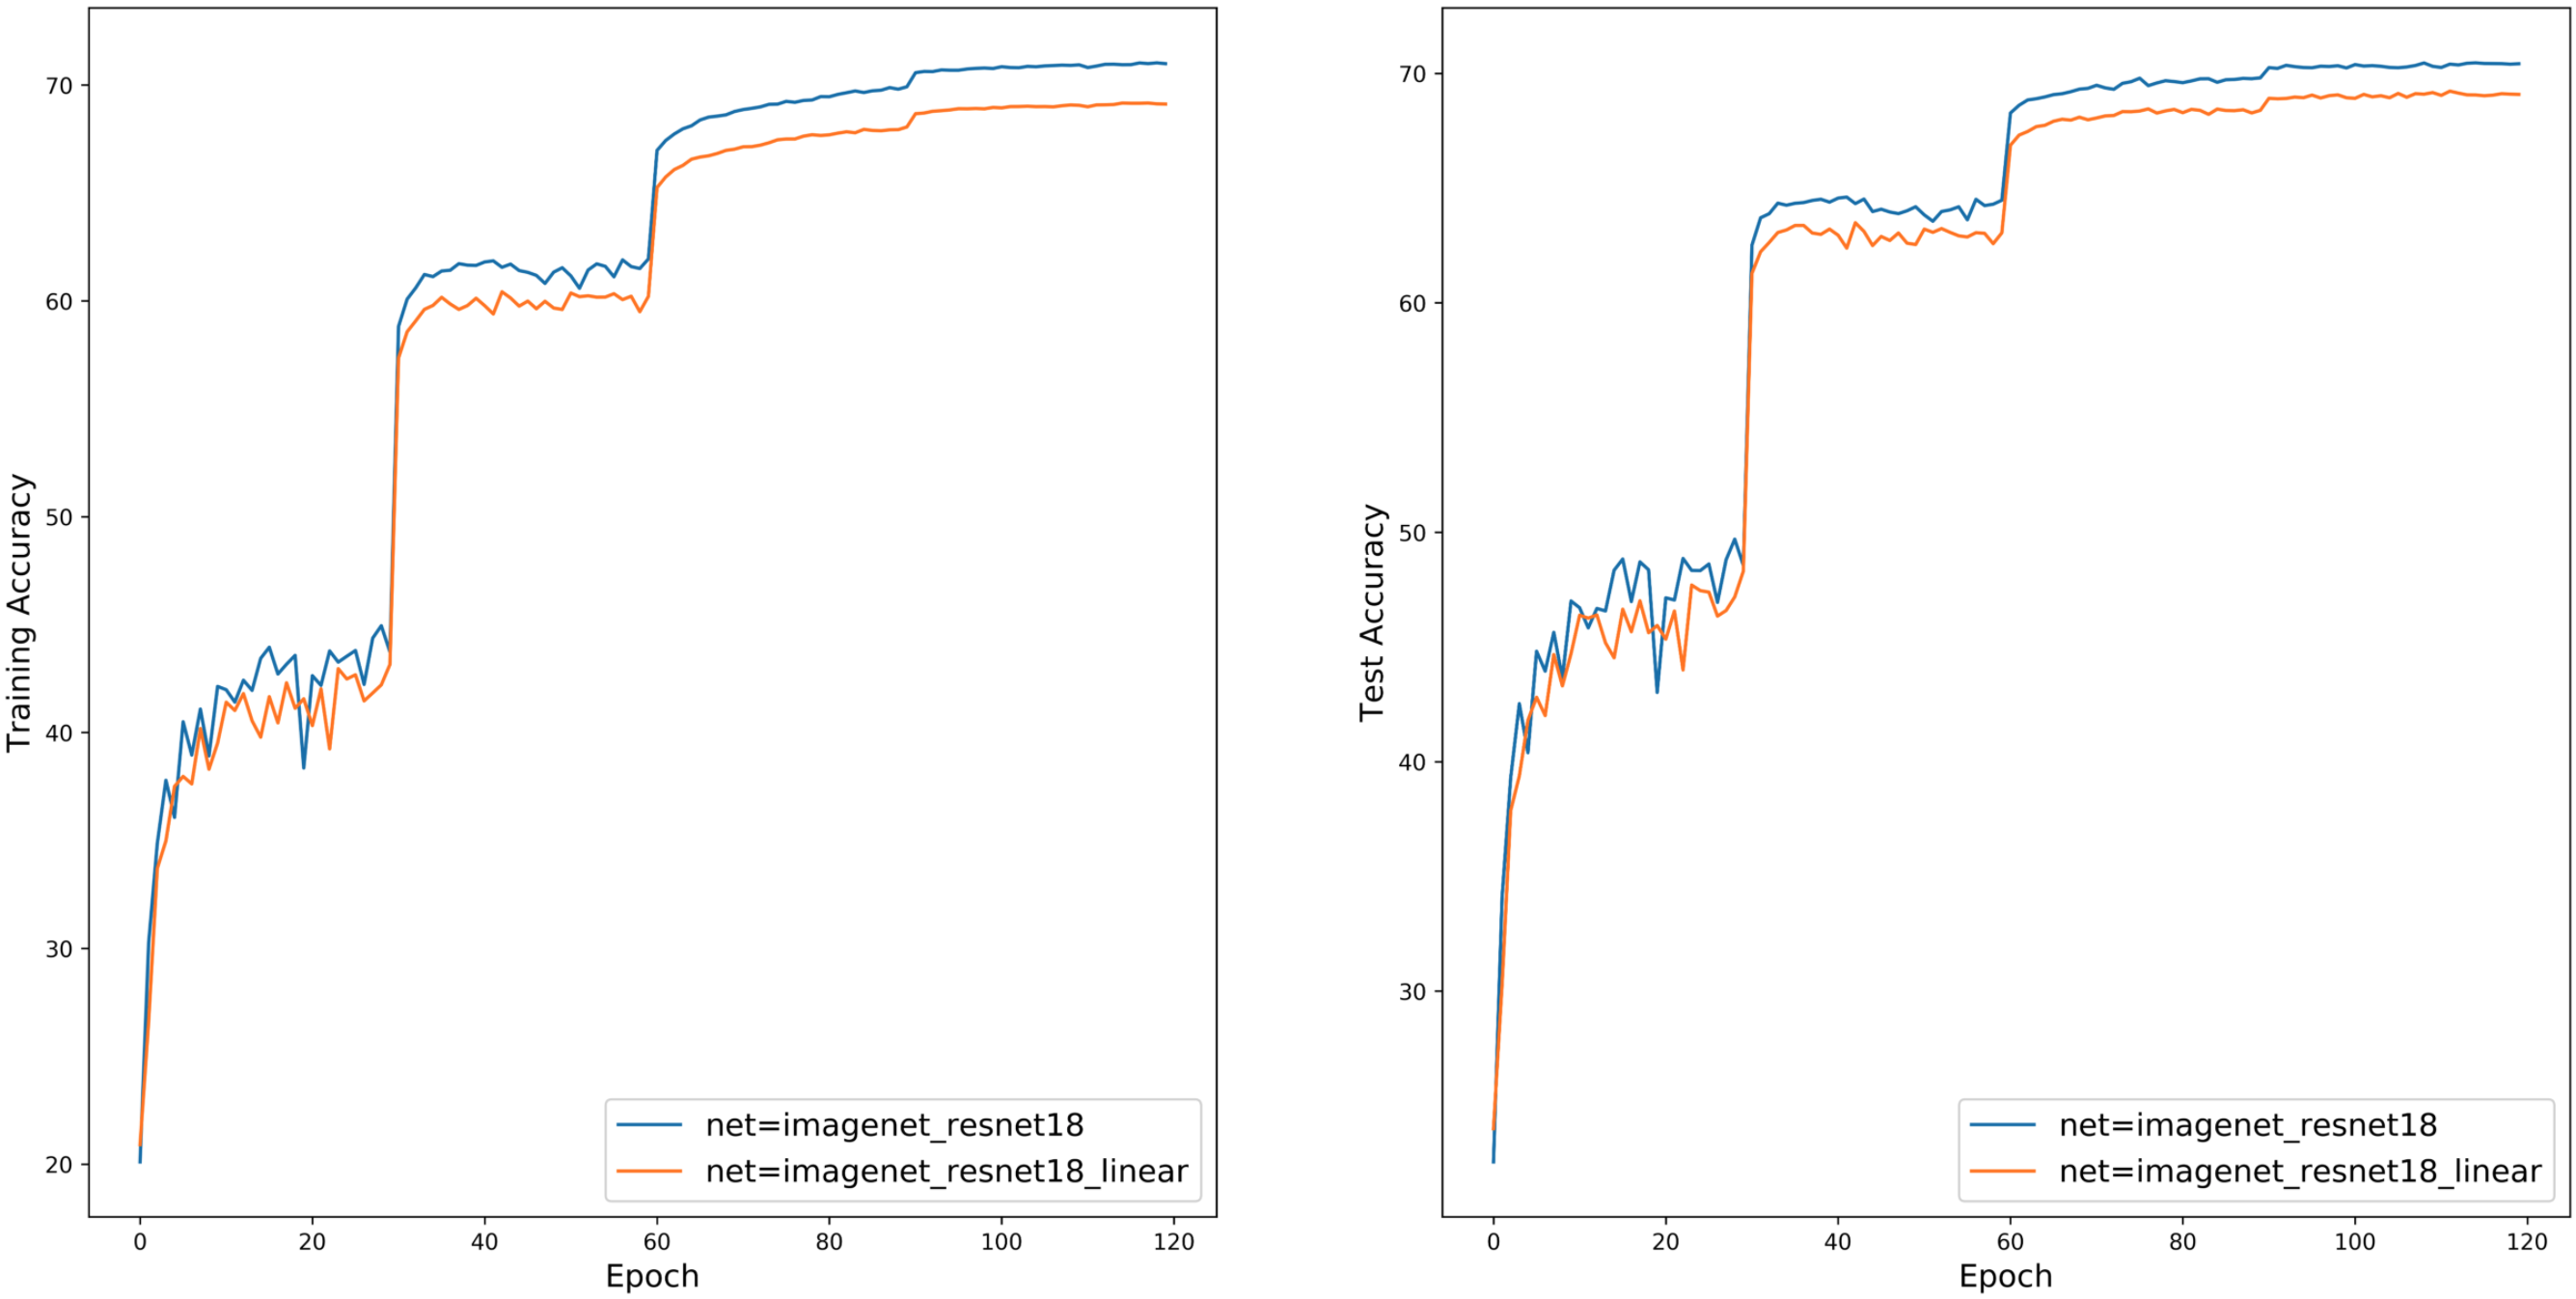
\includegraphics[width=1.2\textwidth]{ImageNetResnet18.png}
	\caption{ResNet18 and ResNet18-$A^l$ on ImageNet.}
	\label{}
\end{figure}
